\documentclass[
  nojss]{jss}

\usepackage[utf8]{inputenc}

\providecommand{\tightlist}{%
  \setlength{\itemsep}{0pt}\setlength{\parskip}{0pt}}

\author{
Johannes Landsheer\\Utrecht University
}
\title{Application of the RPV method and other functions of the
\pkg{UncertainInterval} package}

\Plainauthor{Johannes Landsheer}
\Plaintitle{UncertainInterval: Trichotomous Threshold Determination for Medical
Tests in R}
\Shorttitle{\pkg{UncertainInterval}: Trichotomous Threshold Determination}

\Abstract{
This paper demonstrates the use of the \pkg{UncertainInterval} package
for the determination of an interval of uncertain or inconclusive scores
of medical tests. It is demonstrated using a large synthetic but
realistic data set, with results of the Montreal Cognitive Assessment
(MoCA) for the detection of cognitive impairment (CI). It is shown that
a more robust result can be expected upon avoiding the range of test
scores within which most classification errors are expected, with
adequate predictive values for more clinical settings. The clinical
settings show sample prevalence's of cognitive impairment that vary
widely from .22 to .88. The analysis with the \pkg{UncertainInterval}
package shows a middle range of test scores that does not differentiate
sufficiently between the two true classes of patients. This interval
includes a relatively large part of all errors, when compared to an
optimal dichotomous threshold that minimizes the sum of errors.
Excluding this uncertain or inconclusive range of test scores offers
higher classification accuracies for the samples of individual clinical
settings. In comparison to a dichotomous threshold, excluding the most
error prone test scores enable a classification that offers adequate
accuracies in a larger number of clinical settings.
}

\Keywords{threshold determination, uncertain interval, trichotomization, tests, \proglang{R}}
\Plainkeywords{threshold determination, uncertain interval, trichotomization, tests, R}

%% publication information
%% \Volume{50}
%% \Issue{9}
%% \Month{June}
%% \Year{2012}
%% \Submitdate{}
%% \Acceptdate{2012-06-04}

\Address{
    Johannes Landsheer\\
  Utrecht University\\
  Department Methodology and Statistics, Faculty of Social Sciences
  Padualaan 14, 3584 CH Utrecht\\
  E-mail: \email{j.a.landsheer@uu/nl}\\
  URL: \url{https://www.uu.nl/medewerkers/JALandsheer}\\~\\
  }

% Pandoc header

\usepackage{amsmath}

\begin{document}

\hypertarget{introduction}{%
\section{Introduction}\label{introduction}}

This paper demonstrates the use of the RPV and other functions of the
\pkg{UncertainInterval} package for the determination of test scores
that are uncertain or inconclusive. This results in three classes: a
class of patients with test scores that indicate with a large
probability the absence of the targeted impairment, a class of patients
with test results that are uncertain or inconclusive, and a class of
patients with test scores that most probable indicate the presence of
the targeted impairment. This demonstration uses the test scores of the
Montreal Cognitive Assessment (MoCA) for the screening of cognitive
impairment. The hands-on examples start in paragraph 6.1.

Typically, medical tests are applied to patients who come to a clinical
center for their health complaints via referral or by their own choice.
In contrast to research samples, these patients are not randomly
selected nor can random selection be assumed. Moreover, the population
or sub-populations to which they belong can only be defined by thorough
investigation of their characteristics. In practice, such research is
applied to a part of all patients, a clinical sample that may
demonstrate the characteristics of that population.\\
A medical test is a procedure performed on a patient with a suspected
illness to confirm or determine the presence of the illness. It is
relevant for the determination of the targeted disease to know the
prevalence or proportion of affected individuals within a population.
For the group of patients for whom the disease is suspected, the
probability of the disease is often considerably higher than the
probability of the disease in the general population. For this reason,
the prevalence is often estimated by using the prevalence in the
clinical samples of patients, instead of the (much lower) prevalence in
the general population. Unsurprisingly, these estimates based on
clinical samples can vary widely. The basic question targeted in this
paper is how to deal with widely varying estimates of prevalence. The
method presented does not solve this problem but enables a
classification that offers adequate accuracy in a larger number of
clinical settings.

The screening of patients on the possible presence of a disease forms a
complicated challenge for both primary care physicians and
statisticians. As a running example, data of the Montreal Cognitive
Assessment (MoCA) is used. The MoCA (Montreal Cognitive Assessment) is
considered as one of the best tests for detection of the possible
presence of cognitive impairment in patients. The test has found
world-wide application
\citep{freitas_montreal_2013, larner_screening_2012, martinelli_comparison_2014}.
The results of the test may have serious consequences for the patient,
even when it is only considered as a first step in the diagnostic
process. A false positive may directly lead to cost intensive further
testing and may indirectly lead to loss of independence, which may form
a frightening perspective for the patient. A false negative may prevent
the patient from receiving the help needed to create optimal conditions
of life. A decision for or against the presence of cognitive impairment
is further complicated as the elderly patient may suffer temporary loss
of cognitive abilities due to tiredness, environmental heat, a temporary
illness, or the use of drugs for other diseases
\citep{shiota_temporary_2014}. It is therefore undesirable to jump to
conclusions.\\
The MoCA test is commonly used with a single cutoff score of 26 out of a
maximum of 30, with scores 0 to 25 used for a classification of the
presence of cognitive impairment and a score of 26 to 30 for the
classification of its absence \citep{nasreddine_montreal_2005}. Although
this single cutoff score has been challenged by various researchers
\citep{damian_montreal_2011, davis_montreal_2015, freitas_montreal_2013},
the proposals for alternative cutoff scores remain dichotomized, without
considering the possibility of uncertainty in test outcomes.\\
The model presented here defines three intervals: 1) an interval of
uncertain scores where the patients have about equal probability to be
classified with the targeted disease or not; 2) a lower range of test
scores that indicates the presence of cognitive impairment with high
probability; and 3) an upper range of test scores that indicates normal
cognitive functioning with high probability. In this way, test scores
are trichotomized and interpreted in a way that is straightforward and
can be used without much complications in primary care.\\
On the one hand, this is slightly more complicated than the usual
dichotomization methods \citep{pepe_statistical_2003} that are currently
applied most frequently for medical decision making, including the
determination of possible cognitive impairment. On the other hand, there
are far more sophisticated ways to come to individualized predictions
\citep{sheiner_bayesian_1982}. These methods are often more complicated
\citep{cripps_bayesian_2016}, often do not lead to a single and simple
interpretable rule \citep{logan_decision_2019} or use a `black box'
prediction model that is difficult to explain to clinicians
\citep{logan_decision_2019}. A simpler method may be more practical.\\
Including the commonly used dichotomization methods, any data-based
decision process is a complex form of statistical reasoning, where
multiple population estimates are based on the observed individual
outcomes of a sample of patients (statistical inference) and then these
population estimates are used to interpret the individual patient test
score (statistical syllogism). The population estimates assume that the
results based on other clinical samples will mirror the results of the
sample used in a study.\\
The basics of the most commonly used method (Receiver Operating
Characteristics or ROC) is to consider it as a two-class prediction
problem (binary classification) of two samples of patients for whom the
true status of their illness is known: a sample of patients selected
from the population of patients that are truly affected by the targeted
impairment and a sample of patients selected from the population that is
not affected \citep{pepe_statistical_2003}. The process of selecting the
patients from these two populations requires a measurement that is
superior to the evaluated medical test, known as a binary gold standard
or criterion standard. Subsequently, there are four possible outcomes
when a two-class classifier with a single threshold is used. If the
outcome from a classification is the possible presence of the disease
and the patient is selected form the sample of patients with the
illness, this is called a true positive (TP). When the test result
points to the absence of the impairment for a patient selected from the
sample of patients with the impairment, it is considered a false
positive (FP). A true negative (TN) occurs when the classification
outcome is the absence of the impairment and the patient is selected
from the sample of patients without the impairment, and a false negative
(FN) is found when the classification outcome is the absence of the
impairment while the patient is selected from the sample of patients
that do have the impairment.\\
The common way to find a suitable dichotomous cutoff score is the use of
the receiver operating characteristics of the test, the true positive
rate (\(TPR = Sensitivity = TP / (TP + FN)\)) against the false positive
rate (\(FPR = 1 - Specificity = 1 - TN / (TN + FP)\)), where all
possible test scores are considered as possible thresholds to form two
classes. The original proposal of Nasreddine et
al.~\citeyearpar{nasreddine_montreal_2005} for the dichotomous cutoff
score of the MoCA is based on the balance of sensitivity (\(Se\)) and
specificity (\(Sp\)). A more usual solution is the optimization of the
sum of \(Se\) and \(Sp\), following the proposals of Youden
\citep{youden_index_1950}. This solution also minimizes the sum of the
False Positives (\(FP = 1 - Sp\)) and False Negatives (\(FN = 1 - Se\))
as it minimizes the proportions of the sum of both type of errors
\(Max(Se + Sp) = Min(1 - Sp + 1 - Se)\). It is often considered as the
optimal threshold. The cutoff score that is defined in this way, is
equal to the point of intersection of the densities of the two samples
of patients \citep{schisterman_optimal_2005}. This is the point where
the two samples show no difference in their densities or relative
frequencies, and one might say that the optimal threshold is also the
point where it is impossible to distinguish the two samples based on the
test score alone. In this paper, the optimal threshold is also
considered as the test score that offers maximal classification
uncertainty.\\
Many researchers have argued for the allowance of uncertainty when
interpreting test outcomes, both in the past
\citep{coste_gray_2006, coste_grey_2003, feinstein_inadequacy_1990, greiner_two-graph_1995, simel_intermediate_1987}
and more recently
\citep{hofmann_back_2019, landsheer_interval_2016, landsheer_clinical_2018, schuetz_use_2012, shinkins_diagnostic_2013}.
However, this has not resulted in a change of preferred methods, and
dichotomization using Receiver Operating Characteristics is still the
most used methodology.\\
In this paper, the interval of uncertain test scores is defined as an
interval around the point of intersection in which the densities of the
two samples of patients with and without the targeted impairment are
about the same. The size of this interval is dependent on the quality of
the test (the better the test, the smaller the interval) and the amount
of uncertainty that is allowed. The allowable amount of uncertainty is
of course a subject for discussion.

\hypertarget{data}{%
\section{Data}\label{data}}

\hypertarget{data-set}{%
\subsection{Data set}\label{data-set}}

The original data of 5019 patients is part of the Uniform Data Set
(UDS), collected by the University of Washington's National Alzheimer's
Coordinating Center (NACC) and has been described extensively
\citep{beekly_national_2007, weintraub_alzheimers_2009}. Results of the
original data are available in \citep{Landsheer_In_press}. The results
in this paper are based on an anonymised, synthesized data set
(synthdata\_NACC) that can be published (with the kind permission of the
NACC). The MoCA data has been collected in the period from March 2015 to
August 2018. The test results of 5531 patients at their first visit are
available. Participants were examined in 30 US ADCs. Consent was
obtained at each individual ADC. The subject's cognitive status has been
determined at every visit: normal cognition (NC), cognitively impaired
but not meeting the criteria for MCI, mild cognitive impairment (MCI)
and Dementia. The CDR® Dementia Staging Instrument (CDR) was used
\citep{morris_clinical_1997, morris_clinical_1997-1}) and the global CDR
score was calculated using the defined scoring algorithm. This score is
useful for characterizing a patient's level of cognitive impairment /
dementia, with score 0 indicating normal cognitive functioning.

The original data set is available for researchers from the National
Alzheimer's Coordinating Center
\url{https://www.alz.washington.edu/WEB/nacc_handbook.html}. Also, see
the acknowledgement at the end of the paper.

\hypertarget{gold-standard}{%
\subsection{Gold standard}\label{gold-standard}}

The patients with and without cognitive impairment are defined with
their cognitive status and the global CDR at their first visit to the
ADC. Following Weintraub et al.~\citep{weintraub_version_2018}, the norm
group is defined with a cognitive status of Normal Cognition and a
global CDR score of 0, while the other patients are defined as having
minor or serious cognitive impairment (a cognitive status other than NC
and CDR \textgreater{} 0). Patients who have received an ambiguous
assessment (CDR \textgreater{} 0 and a cognitive status of NC, or a CDR
of 0 and a cognitive status other than NC) have been excluded (n = 512).
Participants in the norm group who achieved low scores on the MoCA were
not removed from the analyses as the patient's status was not defined by
the test. This resulted in a healthy norm group of size 2379 and a group
with a varying level of cognitive impairment of 2640, a total of 5019
patients. The prevalence of cognitive impairment is .53.

\hypertarget{synthesized-example-data}{%
\subsection{Synthesized example data}\label{synthesized-example-data}}

For use as an example, with kind permission of the NACC, a single data
set of 6670 observations from 30 different clinical centers is generated
using the NACC data set as a base. To generate the artificial data, the
\proglang{R} package \pkg{synthpop} \citep{nowok_synthpop_2016} was
used. Results of the real data are available in
\citep{Landsheer_In_press}. Clearly, these example data differs from
those derived from the true NACC data set. Nevertheless, the statistical
results are comparable enough to demonstrate the different methods in
the package \pkg{UncertainInterval}. This data set is named
synthdata\_NACC. The data set contains 8 variables: ID, center, ref.1,
MOCATOTS.1, vdate.1, ref.2, MOCATOTS.2, and vdate.2, respectively
(renumbered) person ID, (renamed) ID of the clinical center, reference
measurement of the true presence of cognitive impairment at the first
measurement, the MoCA total score at the first measurement, the data of
the first measurement, reference measurement of the true presence of
cognitive impairment at the second measurement, the MoCA total score at
the second measurement and the date of the second measurement. At the
first measurement, there are 2433 observations of patients with no
clinical assessment of cognitive impairment and 2644 observations with a
clinical assessment of some form of cognitive impairment.

Researchers who want to use these data for other purposes than
replication of the results presented here, are kindly requested to
submit a new request for the original data to the NACC. The user of the
data may either get a new file or request a file using the
specifications of the original data file
(\url{https://www.alz.washington.edu/}).

\hypertarget{the-problem-of-prevalence}{%
\section{The problem of prevalence}\label{the-problem-of-prevalence}}

The prevalence of a disorder can vary widely between different clinical
institutions. In the original NACC data set, prevalence of cognitive
impairment varied from .22 to .87 for the different centers. In the
total sample, the prevalence was .53. In clinical samples, the patients
are not randomly chosen, but arrive at a clinical center by referral or
by choice. It is therefore difficult to determine a generally valid
estimate of prevalence and clinical samples are difficult to compare
with each other.\\
The optimal cutoff scores for the individual ADCs vary from 19 to 26,
with scores smaller or equal to the optimal cutoff score indicating the
possible presence of cognitive impairment. The optimal cutoff score for
the total sample is 23. When the prevalence is low, the large number of
patients without the impairment results in a large number of patients
that are erroneously classified positive (false positives). When
prevalence is high, a large number of patients with the impairment
receives a negative classification (false negatives). Consequently, the
patterns of incorrect classification differ widely, are strongly
correlated with prevalence and result in a wide variation of negative
and positive predictive values (\(NPV\) and \(PPV\)). The proportion of
correctly classified patients can and will vary dramatically between
clinical settings with different prevalence. In general, prevalence is
strongly positively correlated to the proportion of correctly classified
true patients, and negatively correlated with the proportion of
correctly classified patients without the impairment. Seemingly, this
reflects negatively on the clinical setting, while in reality a
relatively large or small proportion of miss-classifications is due to a
large or small proportion of patients with the impairment.\\
Prevalence has no effect on sensitivity and specificity, provided that
the two patient samples are drawn from the same populations of patients
with and without the targeted condition. This makes sensitivity and
specificity excellent markers of the accuracy of the test, allowing for
the comparison of different samples with varying prevalence and allowing
for comparing different tests using the same sample. It is however
problematic that this does not inform us about the accuracy of the test
result for the patients involved. \(Se\) and \(Sp\) provide information
about the proportion of correctly diagnosed patients, \emph{when given
knowledge about the true status of the patient}. Obviously, this latter
piece of information is not available when a new patient is screened
\citep{gallagher_problem_2003}. Despite the prevalence problems
mentioned above, a positive or negative predictive value (\(PPV\) or
\(NPV\)) provides a clear interpretation for patients: it indicates the
probability of a correct classification, \emph{given the test result}
\citep{gallagher_problem_2003}. Predictive values consequently provide
information about the accuracy of the classification obtained in the
clinical setting.\\
Ransohoff \& Feinstein \citeyearpar{ransohoff_problems_1978} have
stressed that the problem with prevalence is further complicated due to
differences in spectrum bias, when the patients are selected from
various (sub)populations with a different mix of patients. In that case,
varying values can also be expected for \(Se\) and \(Sp\) and these
values can be dependent on prevalence
\citep{brenner_variation_1997, usher-smith_spectrum_2016}.\\
The predictive values (\(PPV\) and \(NPV\)) provide the proportions of
patients classified correctly in the clinical setting and a low
proportion may give reason for concern. Fundamentally, this concern can
be addressed by using better tests, but these may not be available. The
raw classification performance expressed as \(NPV\) and \(PPV\) at one
clinic is not predictive of the classification performance at another
and clinics cannot be compared in this way. A proposal to address this
comparability problem is to use standardized predictive values that
recalculate the predictive values for an assumed prevalence of .5
\citep{heston_standardizing_2011, heston_standardized_2014}.\\
It is difficult to estimate prevalence for clinical samples. It is clear
that patients being tested for a specific disease are not randomly
selected from the general population, but are selected by referral or
self-referral. Furthermore, it is unknown from which (sub)population
they are selected. Heston \citeyearpar{heston_standardized_2014} argued
that as diagnostic tests are most frequently ordered when the diagnosis
is unclear (ie, the pretest likelihood of disease is around 50\%),
standardizing predictive values to a prevalence of 50\% may be more
meaningful to the practicing clinician than estimates based on
prevelance. When doing so, these standardized estimates (\(SNPV\) and
\(SPPV\)) of the predictive values are no more dependent on prevalence
than \(Se\) and \(Sp\) (for dichotomized estimates:
\(SPPV = Se / (Se + 1 - Sp)\) and \(SNPV = Sp / (Sp + 1 - Se))\).\\
In this paper, another way is proposed to lessen the problem of
prevalence. Although it is commonly known that tests offer the best
predictions in the tails and predictions for the test scores in the
middle are far less predictive, this knowledge is seldom applied when
the cutoff scores are determined for the interpretation of the test
results. In such a middle range, a relatively high proportion of
classification errors can be expected. When such a range of uncertain
scores is excluded from a decision for or against the targeted disease,
a relatively large number of errors are prevented, and sufficient
classification results for the scores outside this range can be found
more often.

\hypertarget{managing-uncertain-test-scores}{%
\section{Managing uncertain test
scores}\label{managing-uncertain-test-scores}}

There are different ways to help patients with uncertain test scores.
The first possibility is to apply further tests to reduce the
uncertainty of the classification. This assumes the availability of
another tests that offer additional accuracy. A second possibility is to
await further developments, either by active surveillance or by watchful
waiting \citep{bangma_active_2013}.\\
When a targeted disease is the most serious and the potential
consequences of being left untreated cannot be ignored, while effective
treatment has no serious side effects for patients without the targeted
disease, it is better to choose treatment even in those cases where the
presence of the disease is the most uncertain
\citep{brown_interval_2003, sonis_how_1999}. Treatment possibilities,
benefits and costs of treatment for both correctly classified patients
and for erroneously classified patients are the more relevant when the
classification outcome is uncertain. Knowledge of the inconclusiveness
or uncertainty of the test outcomes can be most helpful for many medical
decisions.

\hypertarget{unstandardized-and-standardized-predictive-values}{%
\section{Unstandardized and standardized predictive
values}\label{unstandardized-and-standardized-predictive-values}}

When the classification problem is defined as a selection problem, the
basic question is whether a patient is selected from the population of
patients with or from the population of patients without the disease.
This question cannot be answered for the individual patient, but it is
possible to estimate the probabilities for the patients that have
obtained a specific test score using Bayesian methods. In the end, the
estimates for groups of patients with a given test score are applied to
the single patient with the same test score. The probability estimates
are derived from multiple population estimates. The desired estimates
are undoubtedly better when the samples used for their estimation are
larger.

\hypertarget{predictive-values}{%
\subsection{Predictive values}\label{predictive-values}}

Predictive values give the probabilities for the presence of the
disease, when the obtained test result is known
\citep{gallagher_problem_2003}. Predictive values therefore provide
information about the accuracy of the classification. Usually the
negative predictive value (\(NPV\)) is calculated for the dichotomized
range of test scores used for a negative classification (test scores
\textgreater{} dichotomous cut-point c), leading to the formulation
\(NPV = TN / (TN + FN)\) and the \(PPV\) for positive classifications
(the range of test scores \textless= c; \(PPV = TP / (TP + FP)\)), where
\(TN\), \(FN\), \(TP\) and \(FP\) concerns the number of respectively
true negative, false negative, true positive and false positive
observations. A more general definition is needed in the context of
three-way classification. Predictive values indicate the likelihood of
the patient's negative and positive real status, given the range of test
scores x. More generally, predictive values are based on the observed
frequencies in the two samples of patients with and without the targeted
disease. For a range of test scores x, if \(f_0(x)\) and \(f_1(x)\) are
the frequencies of patients without and with the targeted disease given
x, the negative predictive value (\(NPV\)) can be defined as:
\(NPV(x) = f_0(x) / (f_0(x) + f_1(x))\) and the positive predictive
value (\(PPV\)) as: \(PPV(x) = f_1(x) / (f_0(x) + f_1(x))\). This
definition also shows that \(NPV(x) = 1 - PPV(x)\) when calculated for
the same range of test scores x.\\
These predictive values are exact for the observed patients with and
without the targeted disease and are valid for the observed sample
prevalence. Interpreting the predictive values of individual test scores
is straightforward. For instance, when 240 true patients from a sample
have score 25, and 257 patients without the targeted disease have score
25 a patient who receives MoCA test score 25, will consequently have a
\(240 / (240 + 257) = 0.48\) probability to belong to the group with CI.
This number is exact for the sample involved. These predictive values
therefore indicate the accuracies of the classifications in the sample,
given the range of applied test score(s). As such, it is an important
outcome for evaluating the accuracy of classification in a sample, given
the observed test score(s). For comparisons of methods, this paper
considers the values of .8 or higher as sufficient, both for \(NPV\) and
\(PPV\).

\hypertarget{standardized-predictive-values.}{%
\subsection{Standardized predictive
values.}\label{standardized-predictive-values.}}

Heston's proposal
\citetext{\citeyear{heston_standardizing_2011}; \citeyear{heston_standardized_2014}}
to standardize predictive values was made in the context of a single
cut-point. However, it makes sense to also use a more general definition
here, and to relate standardized predictive values to the relative
frequencies or densities of the (range of) test score(s). The densities
for a range of test scores x can be defined \(d_0(x) = f_0(x) / n_0\)
and \(d_1(x) = f_1(x) / n_1\), where \(n_0\) and \(n_1\) are the number
of observed patients in the two samples. The standardized negative
predictive value (\(SNPV\)) is defined as
\(SNPV(x) = d_0(x) / (d_0(x) + d_1(x))\) and the standardized positive
predictive value (\(SPPV\)) as \(SPPV(x) = d_1(x) / (d_0(x) + d_1(x))\).
The two distributions are weighted equally, or in other words, the
prevalence is standardized to .5. The interpretation of the standardized
predictive values is not as straightforward as the interpretation of the
common predictive values: they provide the estimated relative
probability which of the two distributions makes the observed test score
most likely, the distribution of the population of patients with or the
population without the disease. If, for instance, 8\% of true patients
have score 25, and 11\% of patients without CI have score 25, a patient
with test score 25 has an estimated relative probability of
\(8 / (8 + 11) = 0.42\) to belong to the population with cognitive
impairment and a probability of 0.58 to belong to the population without
cognitive impairment. The estimates improve with larger samples.
Standardized predictive values can be used to identify the range of
uncertain test scores that offer a limited distinction between the
populations of patients with and without the targeted disease. It should
also be noted that the predictive values of two samples of patients with
and without the targeted impairment (\(PPV\) and \(NPV\)) can be
different from the estimates of the standardized predictive values for
the two populations (\(SPPV\) and \(SNPV\)). These differences are more
substantial when prevalence deviates more strongly from .5.

\hypertarget{post-test-probabilities.}{%
\subsection{Post-test probabilities.}\label{post-test-probabilities.}}

Posttest probabilities \citep{sonis_how_1999} may seem quite different
from predictive values, but they are not. The posttest probability is
equal to the positive predictive value when the pretest probability is
set to the sample prevalence, while the standardized positive predictive
value is equal to the posttest probability when the pretest probability
is set to .5. Post-test probabilities are most versatile, as they can be
calculated for every possible value of prevalence. However, it is
difficult to choose a `correct' prevalence for a patient for whom the
presence of the targeted impairment is unknown, and an assumed pre-test
probability of 0.5 is often the most reasonable. (It should be noted
that Sonis \citeyearpar{sonis_how_1999} discusses a serious disease with
low prevalence for which a relatively harmless and effective cure
exists. It should be clear that in such a case a decision to apply the
cure is easily made, even when the positive test outcome has low
probability and the true presence of the disease is most uncertain.)

\hypertarget{uncertain-test-scores.}{%
\subsection{Uncertain test scores.}\label{uncertain-test-scores.}}

This is defined as a range of test scores with about equal densities in
the two distributions of patients with and without the targeted disease.
Standardized predictive values are therefore most suited to the
determination of this range of uncertain test scores. How much
uncertainty can be allowed is open for discussion. This paper uses an
\(SNPV\) and an \(SPPV\) \textless{} .667 (odds of NCI and CI two to one
or less) to define test scores that are too uncertain for classification
concerning the presence of CI.

\hypertarget{test-reliability-and-smoothing.}{%
\subsection{Test reliability and
smoothing.}\label{test-reliability-and-smoothing.}}

Even if all circumstances remain the same, we cannot expect to find the
same test score for a patient when the same test is taken a second time.
Due to random influences, a second test score will be slightly lower or
higher. Reliable estimates of these predictive probabilities are
consequently needed, and these should be corrected for this randomness
to a certain degree. In test theory, this random effect is estimated
with the Standard Error of Measurement (\(SEM\)), which depends directly
on the reliability of the test: \(SEM = s \sqrt{1 - r}\), where s is the
standard deviation of the test scores and r the estimated reliability of
the test \citep{crocker_introduction_1986, harvill_standard_1991}. The
true score of an individual patient lies with some probability (roughly
68\%) within a range of ±1 \(SEM\) around the observed test score. This
provides information about the range of test scores where the true score
of the patient can be expected. The average standardized predictive
values of a fixed number of consecutive test scores (in this case 5) are
calculated, where each subset of test scores is modified by a forward
shift, excluding the first test score and including the next test score.
Such a moving average smooths the predictive values, stabilizes the
estimates across different samples, and mitigates peculiarities in the
sample. For the determination of thresholds, standardized predictive
values are calculated for the range of ±1 \(SEM\) around each test score
to obtain more stable predictive values.

\hypertarget{determination-of-an-uncertain-interval}{%
\section{Determination of an uncertain
interval}\label{determination-of-an-uncertain-interval}}

The \pkg{UncertainInterval} package has been developed over several
years \citep{landsheer_interval_2016, landsheer_clinical_2018}. Central
to all functions developed for the determination of the uncertain
interval is that in this interval the density is about equal for
patients with and without the targeted disorder. The uncertain interval
is located around the point of intersection of the two density
distributions. Such an uncertain interval is related to the optimal
dichotomous threshold where the sum of the error probabilities
\((1 - Sp + 1 - Se)\) are minimized, which is the same threshold where
the sum \(Se + Sp\) is maximized \citep{youden_index_1950}.\\
The first developed function is \code{ui.nonpar} for the non-parametric
determination of an uncertain interval around the point of intersection
that can be applied to continuous test scores. It iteratively searches
for an interval of test scores around the point of intersection where
these isolated test scores have a given value for both \(Se\) and \(Sp\)
(the default value is .55). Simulation results and an application to a
clinical example are published in Landsheer
\citeyearpar{landsheer_interval_2016}. The clinical example concerns the
prediction of the severity of prostate cancer and is applied to data
published by Hosmer and Lemeshow \citeyearpar{hosmer_jr_applied_2000}.
As \(Se\) and \(Sp\) have been developed as the characteristics of
dichotomization of the full range of observed test scores, the use of
\(Se\) and \(Sp\) as quality indices for limited ranges of test scores
may be counter-intuitive. Commonly used functions for the calculation of
\(Se\) and \(Sp\) do so for the full range of observed test scores.
Therefore, the functions \code{quality.threshold.uncertain} and
\code{quality.threshold} have been created. The function
\code{quality.threshold.uncertain} calculates quality indices for the
range of test scores that form the uncertain interval. When two
thresholds are provided, the function \code{quality.threshold}
calculates the quality indices for the test scores outside the uncertain
interval, ignoring the test scores in the uncertain interval in between
the two thresholds. The functions can also be used for the more usual
calculation of quality indices of the test when applying a single
threshold. The function \code{ui.binormal} is used for the determination
of an uncertain interval when the two distributions of test scores are
assumed to follow a bi-normal distribution. Instead of a search routine,
the function uses an optimization algorithm from the nlopt library
\url{https://nlopt.readthedocs.io/en/latest/NLopt_Algorithms/}: the
sequential quadratic programming (SQP) algorithm for non-linearly
constrained gradient-based optimization (supporting both inequality and
equality constraints), based on the implementation by Kraft
\citetext{\citeyear{kraft_software_1988}; \citeyear{kraft_algorithm_1994}}.
In Landsheer \citeyearpar{landsheer_clinical_2018} simulation results
are published, while the capabilities of the trichotomization method are
demonstrated on an empirical data set published in Andrews and Herzberg
\citeyearpar{andrews_data:_1985} and available in the \proglang{R}
package \pkg{ipred} \citep{peters_cran_2015}. The data set concerns
observations of 75 female Duchenne muscular dystrophy (DMD) carriers and
134 female DMD non-carriers. The various methods are demonstrated for
the serum creatine kinase (CK), marker for the determination of DMD
carriers. The CK marker offers a concordance (AUC or C-statistic) of
0.87. The CK-marker is not the best marker for this determination but
enables the demonstration of the \code{ui.binormal} method. Later, this
function was generalized to cover a wider variety of distributions
different from the bi-normal distribution (function
\code{nl.opt.general}).\\
For comparison, the TG-ROC method of Greiner
\citetext{\citeyear{greiner_two-graph_1995}; \citeyear{greiner_two-graph_1996}}
and the Grey-zone method of Coste et
al.~\citetext{\citeyear{coste_gray_2006}; \citeyear{coste_grey_2003}}
have been used in the two publications
\citep{landsheer_interval_2016, landsheer_clinical_2018}. As the
software for these methods is not generally available, two functions
(\code{TG.ROC} and \code{greyzone}) have been added to the
\pkg{UncertainInterval} package from version 0.5 onwards. These two
methods are also trichotomization methods but differ from the
\pkg{UncertainInterval} methods. Both methods are based on dichotomous
operation characteristics for all possible cutoff-scores of the test.
The resulting middle section of the trichotomization (called
intermediate or greyzone) often overlaps the interval of uncertain test
scores but is not necessarily related to the optimal dichotomous cutoff
score or to equality of densities and can have different properties.
These differences are discussed in Landsheer
\citeyearpar{landsheer_clinical_2018}.

As tests often have discrete scores of interval level, a function has
been added for the exploration of possible uncertain intervals of
ordinal test results (\code{ui.ordinal}). This function can be applied
to small samples of tests with a limited number of ordinal outcomes but
as such it is intended for exploration. Preferably, the determination of
cutoff scores intended for general use should be based on large samples.
When the number of discrete scores is small, \(Se\) and \(Sp\) of a
middle section can vary greatly and a specific value such as the default
value of \(Se\) and \(Sp\) of .55 may be hard to obtain. The
\code{ui.ordinal} function therefore allows for multiple criteria that
can be used for the determination of an inconclusive middle section.\\
The ideas presented by Sonis \citeyearpar{sonis_how_1999} and others
\citep{brown_interval_2003, gallagher_clinical_1998} about interval
likelihood ratios, showed that predictive values, standardized
predictive values, post-test probabilities, as well as interval
likelihood ratios can be used in a straightforward manner for the
determination of the quality indices of intervals of test scores. The
existence of large clinical data sets such as the NACC data set enables
the calculation of these indices for small ranges of test scores, even
when the interval is as small as a single test score. This has resulted
in the \code{RPV} function of the \pkg{UncertainInterval} package, which
calculates predictive values, standardized predictive values, interval
likelihood ratios and posttest probabilities of intervals of test scores
or even the individual test scores of discrete ordinal tests.\\
This paper limits itself to the demonstration of the \code{RPV} function
and several help-functions that are part of the \pkg{UncertainInterval}
package. For the explanation and demonstration of the other functions
see \citep{landsheer_interval_2016, landsheer_clinical_2018} and their
supplemental files and the other vignette in the \pkg{UncertainInterval}
package.

\hypertarget{exploring-the-problem}{%
\subsection{Exploring the problem}\label{exploring-the-problem}}

The first step in the analysis of bi-distributed test scores is the plot
of the distributions. First, we select the first measurements and then
plot these distributions. The \pkg{UncertainInterval} package has two
functions for the purpose: \code{plotMD} and \code{barplotMD}. Both can
be used for ordinal data, but \code{plotMD} is more useful when data are
continuous. The following code loads the package and the example data
set and shows the head and the total number of observations of the data
set.

\begin{CodeChunk}

\begin{CodeInput}
R> library(UncertainInterval)
R> data('synthdata_NACC')
R> head(synthdata_NACC) 
\end{CodeInput}

\begin{CodeOutput}
     ID center ref.1 MOCATOTS.1 vdate.1 ref.2 MOCATOTS.2 vdate.2
14 6411     AD     1          7   16981    NA         NA      NA
36 1079      H     1         21   17095    NA         NA      NA
51 4012      W     0         25   17323    NA         NA      NA
52  785      C    NA         28   17415    NA         NA      NA
70  887      Y    NA         NA      NA     1         22   16772
73 3292      P     1          2   16997    NA         NA      NA
\end{CodeOutput}

\begin{CodeInput}
R> nrow(synthdata_NACC) 
\end{CodeInput}

\begin{CodeOutput}
[1] 6670
\end{CodeOutput}
\end{CodeChunk}

Next, we select the part of data with the first measurements. The gold
standard is defined by two variables (see paragraph 2.2). These two
variables can result in an inconclusive gold standard, which are
excluded:

\begin{CodeChunk}

\begin{CodeInput}
R> m1 = synthdata_NACC[!is.na(synthdata_NACC$MOCATOTS.1) & !is.na(synthdata_NACC$ref.1), ]
\end{CodeInput}
\end{CodeChunk}

Next, check the data for possible missing values and plot the data when
everything is ok:

\begin{CodeChunk}

\begin{CodeInput}
R> addmargins(table(m1$ref.1, m1$MOCATOTS.1, useNA = 'always'))
\end{CodeInput}

\begin{CodeOutput}
      
          0    1    2    3    4    5    6    7    8    9   10   11   12
  0       0    0    0    0    0    0    0    0    0    0    0    0    0
  1       8   13   19   17   20   31   36   47   38   41   52   46   65
  <NA>    0    0    0    0    0    0    0    0    0    0    0    0    0
  Sum     8   13   19   17   20   31   36   47   38   41   52   46   65
      
         13   14   15   16   17   18   19   20   21   22   23   24   25
  0       0    0    4    8   13   16   15   41   49   67  139  208  248
  1      79   98   93   97  134  167  148  170  185  210  191  158  185
  <NA>    0    0    0    0    0    0    0    0    0    0    0    0    0
  Sum    79   98   97  105  147  183  163  211  234  277  330  366  433
      
         26   27   28   29   30 <NA>  Sum
  0     308  414  394  313  199    0 2436
  1     116   82   44   36    6    0 2632
  <NA>    0    0    0    0    0    0    0
  Sum   424  496  438  349  205    0 5068
\end{CodeOutput}

\begin{CodeInput}
R> barplotMD(m1$ref.1, m1$MOCATOTS.1)
\end{CodeInput}


\begin{center}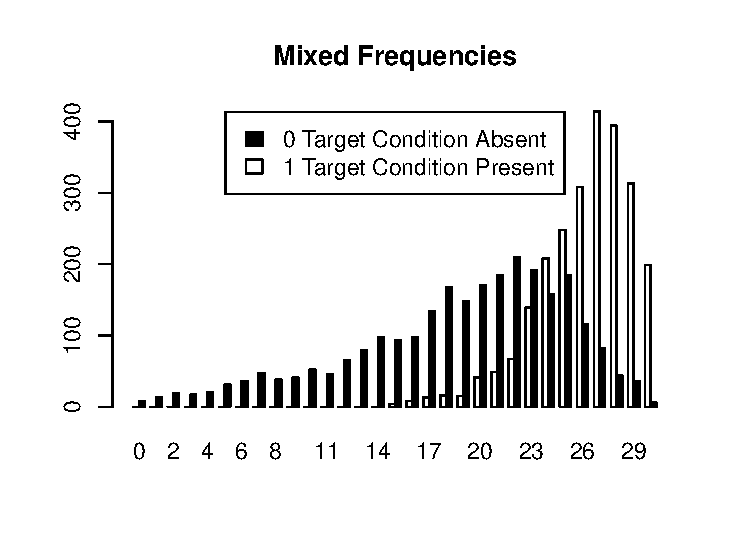
\includegraphics{UI_RPV_files/figure-latex/unnamed-chunk-4-1} \end{center}

\end{CodeChunk}

The bar plot of these realistically simulated data shows the
observations of 2436 patients with no cognitive impairment and 2632
patients with cognitive impairment.

It is easy to see that distinguishing patients with and without
cognitive impairment based on the MoCA test score is relatively easy at
the low end of the test scores: at the low end patients without
cognitive impairment are hardly present. Distinction at the high end of
the test scores is more difficult, as both patients with and without
cognitive impairment can perform quite well on the test and obtain
relatively high test scores.\\
As most functions in the \pkg{UncertainInterval} package assume higher
scores for patients with the targeted condition, the data need to be
negated. This is also the case for the quality functions. When applying
the commonly used cutoff score of 25, with test score 25 and lower
indicating the presence of cognitive impairment, the following results
are obtained.

\begin{CodeChunk}

\begin{CodeInput}
R> quality.threshold(m1$ref.1, -m1$MOCATOTS.1, threshold = -25)
\end{CodeInput}

\begin{CodeOutput}
$table
                       ref
y.hat                      0    1  Sum
  0 (test < threshold)  1628  284 1912
  1 (test >= threshold)  808 2348 3156
  Sum                   2436 2632 5068

$cut
threshold 
      -25 

$indices
                 prevalence correct.classification.rate 
                  0.5193370                   0.7845304 
  balance.correct.incorrect                 specificity 
                  3.6410256                   0.6683087 
                sensitivity   negative.predictive.value 
                  0.8920973                   0.8514644 
  positive.predictive.value                        SNPV 
                  0.7439797                   0.8609880 
                       SPPV        neg.likelihood.ratio 
                  0.7289636                   0.1614564 
       pos.likelihood.ratio                 concordance 
                  2.6895408                   0.8866365 
\end{CodeOutput}
\end{CodeChunk}

The negation of the test scores only influences the table, as the
correct interpretation of the table needs the reversal of the
inequalities: 0 (test score \textgreater{} threshold of 25) and 1 (test
score \textless= 25). The concordance (or AUC) is .89. The Area under
the Curve (AUC) is indicated as concordance in the
\pkg{UncertainInterval} package, as AUC sometimes leads to confusion
about which curve is meant. The correct name is Area under the Receiver
Operating Characteristics Curve or AUROCC. When every possible pair is
formed with one observation from the sample with the disease and one
from the sample of patients without the disease, the AUROCC statistic is
also the concordance between test result and gold standard. The
concordance is the probability that the model correctly ranks all
possible pairs of observations. The name ``concordance'' or C-statistic
for this statistic is therefore also applicable.\\
Although the choice of the creators of the MoCA for this cutoff score of
25 was based on a balance between \(Se\) and \(Sp\), this balance is not
obtained in this clinical sample. The specificity of .67 is quite low.
The optimal Youden threshold is 23 with scores \textless= 23 indicating
Cognitive Impairment. This agrees with the estimated point of
intersection (test scores \textless= 23.54 indicate CI equally well):

\begin{CodeChunk}

\begin{CodeInput}
R> get.intersection(m1$ref.1, -m1$MOCATOTS.1)
\end{CodeInput}

\begin{CodeOutput}
[1] -23.53688
\end{CodeOutput}
\end{CodeChunk}

As the Youden threshold maximizes the sum of \(Se\) + \(Sp\), the
results are slightly better:

\begin{CodeChunk}

\begin{CodeInput}
R> quality.threshold(m1$ref.1, -m1$MOCATOTS.1, threshold = -23)
\end{CodeInput}

\begin{CodeOutput}
$table
                       ref
y.hat                      0    1  Sum
  0 (test < threshold)  2084  627 2711
  1 (test >= threshold)  352 2005 2357
  Sum                   2436 2632 5068

$cut
threshold 
      -23 

$indices
                 prevalence correct.classification.rate 
                  0.5193370                   0.8068272 
  balance.correct.incorrect                 specificity 
                  4.1767109                   0.8555008 
                sensitivity   negative.predictive.value 
                  0.7617781                   0.7687200 
  positive.predictive.value                        SNPV 
                  0.8506576                   0.7821917 
                       SPPV        neg.likelihood.ratio 
                  0.8405574                   0.2784590 
       pos.likelihood.ratio                 concordance 
                  5.2718508                   0.8866365 
\end{CodeOutput}
\end{CodeChunk}

Next, we explore the prevalence of the different centers:

\begin{CodeChunk}

\begin{CodeInput}
R> t = addmargins(table(m1$ref.1, m1$center, useNA = 'always')) 
R> t = rbind(t, t[2,]/(t[2,]+t[1,]))
R> to = t[,c(order(t[5,1:30]),31:32)]
R> rownames(to) = c('0', '1','<NA>','Sum', 'prev')
R> round(to, 3)
\end{CodeInput}

\begin{CodeOutput}
           Q       W      AA       Z       O       L       I       D
0    218.000  89.000 149.000  93.000  89.000 138.000 260.000 119.000
1     60.000  30.000  54.000  34.000  34.000  55.000 112.000  57.000
<NA>   0.000   0.000   0.000   0.000   0.000   0.000   0.000   0.000
Sum  278.000 119.000 203.000 127.000 123.000 193.000 372.000 176.000
prev   0.216   0.252   0.266   0.268   0.276   0.285   0.301   0.324
           X       A      G     AB       M       T       J      R      V
0    114.000  75.000 169.00 55.000 108.000  81.000  90.000 41.000 31.000
1     56.000  42.000 108.00 39.000  84.000  74.000  87.000 46.000 36.000
<NA>   0.000   0.000   0.00  0.000   0.000   0.000   0.000  0.000  0.000
Sum  170.000 117.000 277.00 94.000 192.000 155.000 177.000 87.000 67.000
prev   0.329   0.359   0.39  0.415   0.438   0.477   0.492  0.529  0.537
          P      N       U      AC      F       Y      H       C       E
0    13.000 31.000 105.000  65.000 27.000  40.000  33.00  41.000  34.000
1    16.000 48.000 176.000 123.000 65.000 116.000  99.00 135.000 122.000
<NA>  0.000  0.000   0.000   0.000  0.000   0.000   0.00   0.000   0.000
Sum  29.000 79.000 281.000 188.000 92.000 156.000 132.00 176.000 156.000
prev  0.552  0.608   0.626   0.654  0.707   0.744   0.75   0.767   0.782
           K      AD       S      B <NA>      Sum
0     55.000  50.000  18.000  5.000    0 2436.000
1    284.000 288.000 114.000 38.000    0 2632.000
<NA>   0.000   0.000   0.000  0.000    0    0.000
Sum  339.000 338.000 132.000 43.000    0 5068.000
prev   0.838   0.852   0.864  0.884  NaN    0.519
\end{CodeOutput}

\begin{CodeInput}
R> center = colnames(to)[1:30] # sorted on sample prevalence
\end{CodeInput}
\end{CodeChunk}

The overall prevalence for this sample is .52, but it varies for the
individual centers in this synthesized sample from .22 to .88. Now we
obtain the test indices for the individual centers when the optimal
threshold is applied:

\begin{CodeChunk}

\begin{CodeInput}
R> indm = matrix(NA, 30, 9)
R> yt = rep(NA, 30)
R> for (i in 1:30) {
R+   # i=1
R+   ref = m1[m1$center == center[i], ]$ref.1 
R+   unique(ref)
R+   test = -m1[m1$center == center[i], ]$MOCATOTS.1
R+   N0 = length(test[ref == 0])
R+   N1 = length(test[ref == 1])
R+   indm[i, ] = c(N0, N1,
R+                 quality.threshold(ref, test, threshold = -23, 
R+                    model = 'ordinal')$indices[c(1, 4:9)])
R+ }
R> colnames(indm) = c('n0', 'n1', 'prev', 'Sp', 'Se', 'NPV', 'PPV', 'SNPV', 'SPPV')
R> rownames(indm) = 1:30
R> round(indm, 3)
\end{CodeInput}

\begin{CodeOutput}
    n0  n1  prev    Sp    Se   NPV   PPV  SNPV  SPPV
1  218  60 0.216 0.899 0.967 0.990 0.725 0.964 0.905
2   89  30 0.252 0.798 0.500 0.826 0.455 0.615 0.712
3  149  54 0.266 0.852 0.889 0.955 0.686 0.885 0.858
4   93  34 0.268 0.849 0.794 0.919 0.659 0.805 0.841
5   89  34 0.276 0.910 0.824 0.931 0.778 0.838 0.902
6  138  55 0.285 0.964 0.655 0.875 0.878 0.736 0.948
7  260 112 0.301 0.888 0.759 0.895 0.746 0.787 0.872
8  119  57 0.324 0.706 0.860 0.913 0.583 0.834 0.745
9  114  56 0.329 0.868 0.768 0.884 0.741 0.789 0.854
10  75  42 0.359 0.867 0.357 0.707 0.600 0.574 0.728
11 169 108 0.390 0.734 0.741 0.816 0.640 0.739 0.736
12  55  39 0.415 1.000 0.385 0.696 1.000 0.619 1.000
13 108  84 0.438 0.759 0.714 0.774 0.698 0.727 0.748
14  81  74 0.477 0.741 0.865 0.857 0.753 0.846 0.769
15  90  87 0.492 0.900 0.805 0.827 0.886 0.822 0.889
16  41  46 0.529 1.000 0.652 0.719 1.000 0.742 1.000
17  31  36 0.537 0.903 0.500 0.609 0.857 0.644 0.838
18  13  16 0.552 0.538 0.938 0.875 0.714 0.896 0.670
19  31  48 0.608 0.806 0.771 0.694 0.860 0.779 0.799
20 105 176 0.626 0.781 0.835 0.739 0.865 0.826 0.792
21  65 123 0.654 0.877 0.829 0.731 0.927 0.837 0.871
22  27  65 0.707 0.778 0.769 0.583 0.893 0.771 0.776
23  40 116 0.744 0.925 0.767 0.578 0.967 0.799 0.911
24  33  99 0.750 0.909 0.747 0.545 0.961 0.783 0.892
25  41 135 0.767 0.976 0.593 0.421 0.988 0.705 0.960
26  34 122 0.782 0.824 0.910 0.718 0.949 0.901 0.838
27  55 284 0.838 0.909 0.761 0.424 0.977 0.792 0.893
28  50 288 0.852 1.000 0.851 0.538 1.000 0.870 1.000
29  18 114 0.864 0.833 0.693 0.300 0.963 0.731 0.806
30   5  38 0.884 1.000 0.500 0.208 1.000 0.667 1.000
\end{CodeOutput}
\end{CodeChunk}

The centers are sorted on the prevalence of CI found in their data. The
following matrix shows the correlations between prevalence and the
various quality indices:

\begin{CodeChunk}

\begin{CodeInput}
R> round(cor(indm[,'prev'], indm[,c('NPV', 'PPV', 'Sp', 'Se', 'SNPV', 'SPPV')]), 2)
\end{CodeInput}

\begin{CodeOutput}
       NPV  PPV   Sp    Se SNPV SPPV
[1,] -0.87 0.77 0.19 -0.01    0 0.26
\end{CodeOutput}
\end{CodeChunk}

The correlations between prevalence and \(Sp\) and \(Se\) are low. As
expected, the correlations between prevalence and \(NPV\) and \(PPV\)
are considerable (-.87 and .77), while the correlations with their
standardized version \(SNPV\) and \(SPPV\) are about as low as the
correlations with \(Sp\) and \(Se\).

The MoCA has inadequate test accuracy indices (\(Se\) and \(Sp\)) for
some of the centers. The following command line shows the line numbers
in table \code{indm}:

\begin{CodeChunk}

\begin{CodeInput}
R> which(indm[,'Se'] < .7)
\end{CodeInput}

\begin{CodeOutput}
 2  6 10 12 16 17 25 29 30 
 2  6 10 12 16 17 25 29 30 
\end{CodeOutput}

\begin{CodeInput}
R> which(indm[,'Sp'] < .7)
\end{CodeInput}

\begin{CodeOutput}
18 
18 
\end{CodeOutput}
\end{CodeChunk}

It is noteworthy that low sensitivity is found both for centers with low
prevalence and for centers with high prevalence of CI. The low
Specificity results occur for an center with a prevalence of .552.
Clearly, the MoCA does not function equally well for all centers and
this should receive more attention (it should be noted that similar
results are also obtained for the real data).

Dependent on prevalence, the percentages of correctly classified
patients can be quite low. When a lower limit of .8 is used (4 out of 5
patients classified correctly), mainly centers with low prevalence show
sufficient values for \(NPV\), while mainly centers with high prevalence
show sufficient values for \(PPV\).

\begin{CodeChunk}

\begin{CodeInput}
R> which(indm[,'NPV'] >= .8)
\end{CodeInput}

\begin{CodeOutput}
 1  2  3  4  5  6  7  8  9 11 14 15 18 
 1  2  3  4  5  6  7  8  9 11 14 15 18 
\end{CodeOutput}

\begin{CodeInput}
R> which(indm[,'PPV'] >= .8)
\end{CodeInput}

\begin{CodeOutput}
 6 12 15 16 17 19 20 21 22 23 24 25 26 27 28 29 30 
 6 12 15 16 17 19 20 21 22 23 24 25 26 27 28 29 30 
\end{CodeOutput}

\begin{CodeInput}
R> which(indm[,'PPV'] >= .8 & indm[,'NPV'] >= .8)
\end{CodeInput}

\begin{CodeOutput}
 6 15 
 6 15 
\end{CodeOutput}
\end{CodeChunk}

Only for 2 centers, both the value for \(NPV\) and \(PPV\) are
\textgreater= .8.

\hypertarget{determination-of-an-uncertain-interval-1}{%
\subsection{Determination of an uncertain
interval}\label{determination-of-an-uncertain-interval-1}}

As explained earlier, we first need the test reliability to enable
smoothing of the distributions and obtaining more stable estimates. The
time \code{ddiff} between measurements varies widely. The reliability is
estimated with the \code{ICC} function of the \pkg{psych} package.

\begin{CodeChunk}

\begin{CodeInput}
R> ddiff = (m1$vdate.2 - m1$vdate.1)
R> summary(ddiff)
\end{CodeInput}

\begin{CodeOutput}
   Min. 1st Qu.  Median    Mean 3rd Qu.    Max.    NA's 
   62.0   363.0   385.0   423.3   455.0  1063.0    3192 
\end{CodeOutput}

\begin{CodeInput}
R> library(psych)
R> ICC(na.omit(cbind(m1$MOCATOTS.1, m1$MOCATOTS.2)))
\end{CodeInput}

\begin{CodeOutput}
Call: ICC(x = na.omit(cbind(m1$MOCATOTS.1, m1$MOCATOTS.2)))

Intraclass correlation coefficients 
                         type  ICC  F  df1  df2 p lower bound upper bound
Single_raters_absolute   ICC1 0.86 14 1875 1876 0        0.85        0.87
Single_random_raters     ICC2 0.86 14 1875 1875 0        0.84        0.88
Single_fixed_raters      ICC3 0.87 14 1875 1875 0        0.86        0.88
Average_raters_absolute ICC1k 0.93 14 1875 1876 0        0.92        0.93
Average_random_raters   ICC2k 0.93 14 1875 1875 0        0.91        0.94
Average_fixed_raters    ICC3k 0.93 14 1875 1875 0        0.92        0.94

 Number of subjects = 1876     Number of Judges =  2
\end{CodeOutput}
\end{CodeChunk}

Over all, \code{ICC} is .86 for the subjects that have two measurements.
The intended distance between the meausurements of the UDS is one year
apart. When selecting the patients whose second measurements are between
11 and 13 months apart (335 and 395 days apart), 917 observations
remain:

\begin{CodeChunk}

\begin{CodeInput}
R> timesel = (ddiff >= 335) & (ddiff <= 395)
R> ICC(na.omit(cbind(m1$MOCATOTS.1[timesel], m1$MOCATOTS.2[timesel])))
\end{CodeInput}

\begin{CodeOutput}
Call: ICC(x = na.omit(cbind(m1$MOCATOTS.1[timesel], m1$MOCATOTS.2[timesel])))

Intraclass correlation coefficients 
                         type  ICC  F df1 df2        p lower bound
Single_raters_absolute   ICC1 0.87 15 916 917 1.4e-287        0.86
Single_random_raters     ICC2 0.87 15 916 916 8.2e-292        0.85
Single_fixed_raters      ICC3 0.88 15 916 916 8.2e-292        0.86
Average_raters_absolute ICC1k 0.93 15 916 917 1.4e-287        0.92
Average_random_raters   ICC2k 0.93 15 916 916 8.2e-292        0.92
Average_fixed_raters    ICC3k 0.93 15 916 916 8.2e-292        0.92
                        upper bound
Single_raters_absolute         0.89
Single_random_raters           0.89
Single_fixed_raters            0.89
Average_raters_absolute        0.94
Average_random_raters          0.94
Average_fixed_raters           0.94

 Number of subjects = 917     Number of Judges =  2
\end{CodeOutput}

\begin{CodeInput}
R> # ICC(na.omit(cbind(m1$MOCATOTS.1[timesel], m1$MOCATOTS.2[timesel])), lmer=FALSE)
\end{CodeInput}
\end{CodeChunk}

The lower estimate (.86) is chosen as the reliability estimate. The
\code{RPV} function calculates predictive values, interval likelihood
ratios and post-test probabilities of individual test scores for
discrete ordinal tests. The function also trichotomizes the test
results, with an uncertain interval where the test scores do not allow
for an adequate distinction between the two groups of patients. To
reduce random effects, the standardized predictive values are calculated
for a range of scores around the obtained score. As the default
calculated range of scores is uneven, the function returns an error and
proposes suitable values for the parameter \code{roll.length} that
determines the ranges of test scores. In the following command,
\code{roll.length} is set to 5.

\begin{CodeChunk}

\begin{CodeInput}
R> RPV(m1$ref.1, m1$MOCATOTS.1, reliability = .86, roll.length = 5)
\end{CodeInput}

\begin{CodeOutput}
$parameters
     pretest.prob sample.prevalence       reliability               SEM 
            0.519             0.519             0.860             2.310 
      roll.length    rel.conf.level     decision.odds             limit 
            5.000             0.613             2.000             0.667 

$messages
     [,1]                                                                   
[1,] "Reliable Predictive Values for scores  0 1 29 30  have been extended."
[2,] "Decision use = standardized.pv."                                      

$rel.pred.values
           0   1   2   3   4   5   6   7   8   9  10  11  12     13     14
rnpv       0   0   0   0   0   0   0   0   0   0   0   0   0  0.010  0.027
rppv       1   1   1   1   1   1   1   1   1   1   1   1   1  0.990  0.973
rsnpv      0   0   0   0   0   0   0   0   0   0   0   0   0  0.011  0.029
rsppv      1   1   1   1   1   1   1   1   1   1   1   1   1  0.989  0.971
rilr     Inf Inf Inf Inf Inf Inf Inf Inf Inf Inf Inf Inf Inf 88.157 33.319
rpt.odds Inf Inf Inf Inf Inf Inf Inf Inf Inf Inf Inf Inf Inf 95.250 36.000
rpt.prob   1   1   1   1   1   1   1   1   1   1   1   1   1  0.990  0.973
             15     16     17    18    19    20    21    22    23    24
rnpv      0.048  0.065  0.081 0.115 0.143 0.176 0.256 0.355 0.434 0.530
rppv      0.952  0.935  0.919 0.885 0.857 0.824 0.744 0.645 0.566 0.470
rsnpv     0.051  0.070  0.086 0.123 0.153 0.188 0.271 0.373 0.453 0.549
rsppv     0.949  0.930  0.914 0.877 0.847 0.812 0.729 0.627 0.547 0.451
rilr     18.548 13.296 10.561 7.126 5.553 4.332 2.690 1.678 1.209 0.821
rpt.odds 20.040 14.366 11.411 7.699 6.000 4.681 2.907 1.813 1.307 0.887
rpt.prob  0.952  0.935  0.919 0.885 0.857 0.824 0.744 0.645 0.566 0.470
            25    26    27    28    29    30
rnpv     0.643 0.729 0.784 0.851 0.851 0.851
rppv     0.357 0.271 0.216 0.149 0.149 0.149
rsnpv    0.660 0.744 0.796 0.861 0.861 0.861
rsppv    0.340 0.256 0.204 0.139 0.139 0.139
rilr     0.514 0.344 0.256 0.161 0.161 0.161
rpt.odds 0.556 0.372 0.276 0.174 0.174 0.174
rpt.prob 0.357 0.271 0.216 0.149 0.149 0.149

$result
                  Negative Decisions Uncertain Positive Decisions
scores            26-30              22-25     0-21              
n                 1912               1406      1750              
total.sample      37.7%              27.7%     34.5%             
correct.decisions 85.1%              NA%       91.7%             
true.neg.status   66.8%              27.2%     6.0%              
true.pos.status   10.8%              28.3%     60.9%             
realized.odds     5.732              1.124     10.986            
\end{CodeOutput}
\end{CodeChunk}

The parameters of the analysis are presented in \code{\$parameters}. The
size of this range is set to (approximate) the score ±1 \(SEM\). The
estimate of \(SEM\) is 2.305. The selected \code{roll.length = 5} sets
the ranges of the test score ± 2 and the results are the moving averages
of the test scores ± 2. This covers a confidence level of 61.4\% for the
expected true test score. The calculated results are the moving averages
over these ranges. Applying the odds of a correct classification as 2
against 1 means the lower limit of \(SNPV\) or \(SPPV\) is .667 and test
scores that offer either an \(SNPV\) or \(SPPV\) lower than .667 are
considered as inconclusive or uncertain.

Reliable standardized predictive values cannot be calculated for the
most extreme values (test scores 0, 1, 29 and 30) and are consequently
extended from the nearest calculable value. This is reported in
\code{\$messages}. The test scores at the extremes of the test results
represent the highest and lowest standardized predictive values. In
practice, this extension should therefore rarely pose a problem for the
determination of the most uncertain test scores, as classification
errors are typically found around the Youden threshold (in this case 23)
and not in the tails of the distributions.\\
Various statistics are shown in \code{\$rel.pred.values}. It shows the
smoothed predictive values (\code{rnpv} and \code{rppv}), the density
based standardized negative and positive predictive values (\code{rsnpv}
and \code{rsppv}), the interval likelihood ratios (\code{rilnr}), the
posttest odds (\code{rpt.odds}) and the posttest probabilities
(\code{rpt.prob}). In this case, \code{rpt.prob} equals \code{rppv} as
the prevalence is kept equal to the sample prevalence.\\
The standardized negative and positive predictive values are used for
the decision thresholds. In this case, \code{rpt.prob} equals
\code{rppv} as the prevalence is kept equal to the sample prevalence as
a default. The standardized predictive values are equal to the posttest
probabilities when prevalence is set to .5. The decision results are
shown in \code{$result}. The determined uncertain interval is 22 to 25,
which contains 27.2\% of patients with a true negative status and 28.3\%
of the patients with a true positive status. The realized decision odds
for the uncertain interval are 1.124 which means that the ratio of the
densities of patients with and without cognitive impairment
\(d_1(x) / d_0(x)\) is close to 1. The range 26-30 is selected for
negative decisions which results in 85.1\% correct decisions and covers
66.8\% of the patients with a true negative status. The range 0-21 is
selected for positive decisions. It has a percentage of 91.7 of correct
decisions and covers 60.9\% patients with a true positive status.\\
Although the uncertain interval contains 27.7\% of the total sample, no
less than 56\% of all errors are found here when the optimal threshold
(23) would have been applied:

\begin{CodeChunk}

\begin{CodeInput}
R> class23 = as.numeric(m1$MOCATOTS.1 <= 23)
R> err = m1$ref.1 != class23
R> sum(err[m1$MOCATOTS.1 >= 22 & m1$MOCATOTS.1 <= 25])/ sum(err)
\end{CodeInput}

\begin{CodeOutput}
[1] 0.5607763
\end{CodeOutput}
\end{CodeChunk}

The results of this trichotomization for the individual centers are:

\begin{CodeChunk}

\begin{CodeInput}
R> indm2 = matrix(NA, 30, 4); i=1
R> for (i in 1:30){
R+   ref = m1[m1$center==center[i],]$ref.1
R+   test = m1[m1$center==center[i],]$MOCATOTS.1 # reversed order
R+   res = RPV(ref, test, pretest.prob = .53, reliability=.86, roll.length=5,
R+             decision.odds = 2, preselected.thresholds = c(25,22))$result[4:6,]
R+   res2=c(t(res))[c(1,3,4,9)]
R+   indm2[i,] = as.numeric(c(sub("%","",res2[1]), sub("%","",res2[2]),
R+                           sub("%","",res2[3]),sub("%","",res2[4])))/100
R+ }
R> indm2=cbind(to['prev',1:30], indm2)
R> colnames(indm2) = c('prev', 'NPV', 'PPV', 'Sp', 'Se')
R> # SPPV = Se / (Se + 1 – Sp) and SNPV = Sp / (Sp + 1 – Se)).
R> SNPV = indm2[,'Sp']/(indm2[,'Sp']+ 1 - indm2[,'Se'])
R> SPPV = indm2[,'Se']/(indm2[,'Se']+ 1 - indm2[,'Sp'])
R> rownames(indm2)= 1:30
R> indm2 = cbind(indm2, SNPV, SPPV)
R> round(indm2, 3)
\end{CodeInput}

\begin{CodeOutput}
    prev   NPV   PPV    Sp    Se  SNPV  SPPV
1  0.216 1.000 0.833 0.711 0.750 0.740 0.722
2  0.252 0.919 0.478 0.640 0.367 0.503 0.505
3  0.266 0.940 0.860 0.631 0.685 0.667 0.650
4  0.268 0.969 0.893 0.667 0.735 0.716 0.688
5  0.276 0.950 0.958 0.640 0.676 0.664 0.653
6  0.285 0.927 0.875 0.826 0.382 0.572 0.687
7  0.301 0.892 0.855 0.638 0.580 0.603 0.616
8  0.324 0.985 0.725 0.538 0.649 0.605 0.584
9  0.329 0.940 0.943 0.684 0.589 0.625 0.651
10 0.359 0.844 0.750 0.720 0.286 0.502 0.505
11 0.390 0.869 0.739 0.550 0.630 0.598 0.583
12 0.415 0.750 1.000 0.982 0.256 0.569 0.934
13 0.438 0.909 0.727 0.463 0.571 0.519 0.515
14 0.477 0.887 0.957 0.580 0.608 0.597 0.591
15 0.492 0.833 0.934 0.556 0.655 0.617 0.596
16 0.529 0.800 1.000 0.878 0.522 0.647 0.811
17 0.537 0.743 1.000 0.839 0.361 0.568 0.692
18 0.552 1.000 0.789 0.308 0.938 0.832 0.575
19 0.608 0.792 0.933 0.613 0.583 0.595 0.601
20 0.626 0.847 0.917 0.686 0.750 0.733 0.705
21 0.654 0.930 0.958 0.615 0.748 0.709 0.660
22 0.707 0.808 1.000 0.778 0.631 0.678 0.740
23 0.744 0.756 0.971 0.775 0.586 0.652 0.723
24 0.750 0.769 0.981 0.606 0.515 0.555 0.567
25 0.767 0.547 0.984 0.854 0.459 0.612 0.759
26 0.782 1.000 0.968 0.735 0.738 0.737 0.736
27 0.838 0.595 0.982 0.909 0.581 0.684 0.865
28 0.852 0.611 1.000 0.880 0.729 0.765 0.859
29 0.864 0.316 0.984 0.333 0.535 0.417 0.445
30 0.884 0.400 1.000 0.800 0.395 0.569 0.664
\end{CodeOutput}
\end{CodeChunk}

The correlations between the predictive values and prevalence are
reduced but still considerable:

\begin{CodeChunk}

\begin{CodeInput}
R> round(cor(indm2[,'prev'], 
R+           indm2[,c('NPV', 'PPV', 'Sp', 'Se', 'SNPV', 'SPPV')]), 2)
\end{CodeInput}

\begin{CodeOutput}
       NPV  PPV   Sp   Se SNPV SPPV
[1,] -0.72 0.59 0.16 0.04 0.07 0.24
\end{CodeOutput}
\end{CodeChunk}

However, there is an increase in the number of centers with sufficient
classification accuracy:

\begin{CodeChunk}

\begin{CodeInput}
R> which(indm2[,'NPV'] >= .8)
\end{CodeInput}

\begin{CodeOutput}
 1  2  3  4  5  6  7  8  9 10 11 13 14 15 16 18 20 21 22 26 
 1  2  3  4  5  6  7  8  9 10 11 13 14 15 16 18 20 21 22 26 
\end{CodeOutput}

\begin{CodeInput}
R> which(indm2[,'PPV'] >= .8)
\end{CodeInput}

\begin{CodeOutput}
 1  3  4  5  6  7  9 12 14 15 16 17 19 20 21 22 23 24 25 26 27 28 29 30 
 1  3  4  5  6  7  9 12 14 15 16 17 19 20 21 22 23 24 25 26 27 28 29 30 
\end{CodeOutput}

\begin{CodeInput}
R> which(indm2[,'PPV'] >= .8 & indm2[,'NPV'] >= .8)
\end{CodeInput}

\begin{CodeOutput}
 1  3  4  5  6  7  9 14 15 16 20 21 22 26 
 1  3  4  5  6  7  9 14 15 16 20 21 22 26 
\end{CodeOutput}
\end{CodeChunk}

There are now 20 centers with \(NPV\) \textgreater= .8 and 24 centers
with \(PPV\) \textgreater= .8. For both \(PPV\) and \(NPV\), 14 centers
can use the MoCA in this manner to classify both patients with and
without CI correctly in at least 4 out of 5 cases.

The results for \(Sp\) and \(Se\) are lower compared to the table based
on the optimal dichotomization. This is because for the calculation of
\(Sp\) and \(Se\), the uncertain test scores are all incorrectly
considered as unambiguous errors. Especially when using these uncertain
scores for a positive or negative classification, many classification
errors are made. When these test scores are considered as uncertain,
another possible line of action can be chosen. In these cases, choosing
a more cautious line of action can reduce over-treatment and treatment
errors.

The indices \(Se\) and \(Sp\) are meant for a dichotomous classification
and are cumbersome to apply when using a three-way classification. A
possible alternative is ignoring the uncertain test scores (function
\code{quality.uncertain}) for the calculation of the test indices.

\hypertarget{alternative-software}{%
\section{Alternative software}\label{alternative-software}}

Trichotomization software is scarce. The earlier developed software for
the Two-Graphs receiver Operating Characteristics
\citep{greiner_two-graph_1995, greiner_two-graph_1996} is no longer
available. A non-parametric implementation of function \code{TGROC} is
available in package (\pkg{DiagnosisMed}, which is under development
\citep{brasil_diagnosismed_2018}. For the Grey zone method
\citep{coste_gray_2006, coste_grey_2003} software is not available. Both
a \code{TG-ROC} and a \code{greyzone} function have been made part of
the \pkg{UncertainInterval} package.\\
I also like to point to an alternative \proglang{R} package for
trichotomization: \pkg{ThreshholdROC}
\citep{perez-jaume_thresholdroc:_2017}. This method is most suitable
when there are three distinguishable underlying states and is especially
suitable for tests that allow for a finer distinction. When underlying
states are less easy to distinguish in three different states, a middle
range of test scores is better considered as uncertain and the package
\pkg{UncertainInterval} may be a better choice.

\hypertarget{discussion}{%
\section{Discussion}\label{discussion}}

The \pkg{UncertainInterval} package allows for the identification of a
middle range of uncertain test scores. The main advantage is that it
enables identification of test scores that have about equal likelihood
of identifying a patient with or without the targeted impairment. The
application on the MoCA shows that a large number of classification
errors are prevented when considering these test scores as uncertain.
Choosing a more cautious line of action such as awaiting further
developments while applying active surveillance or watchful waiting is
considered best practice for a disease such as prostate cancer
\citep{bangma_active_2013}. Knowing which range of test scores are
inconclusive concerning the targeted disease may help in considering
benefits and costs both for patients with and without the targeted
disease.\\
This paper also shows a secondary benefit of considering a range of test
scores as uncertain: it allows the application of trichotomized cutoff
scores that can be applied in a wider range of clinical settings as they
offer sufficient classification accuracy in more settings that vary in
the mix of patients with and without the targeted disease. While this
does not solve the problem of prevalence, it does alleviate it.

\hypertarget{acknowledgement}{%
\section{Acknowledgement}\label{acknowledgement}}

The NACC database is funded by NIA/NIH Grant U01 AG016976. NACC data are
contributed by the NIA funded ADCs: P30 AG019610 (PI Eric Reiman, MD),
P30 AG013846 (PI Neil Kowall, MD), P50 AG008702 (PI Scott Small, MD),
P50 AG025688 (PI Allan Levey, MD, PhD), P50 AG047266 (PI Todd Golde, MD,
PhD), P30 AG010133 (PI Andrew Saykin, PsyD), P50 AG005146 (PI Marilyn
Albert, PhD), P50 AG005134 (PI Bradley Hyman, MD, PhD), P50 AG016574 (PI
Ronald Petersen, MD, PhD), P50 AG005138 (PI Mary Sano, PhD), P30
AG008051 (PI Steven Ferris, PhD), P30 AG013854 (PI M. Marsel Mesulam,
MD), 30 AG008017 (PI Jeffrey Kaye, MD), P30 AG010161 (PI David Bennett,
MD), P50 AG047366 (PI Victor Henderson, MD, MS), P30 AG010129 (PI
Charles DeCarli, MD), P50 AG016573 (PI Frank LaFerla, PhD), P50 AG016570
(PI Marie-Francoise Chesselet, MD, PhD), P50 AG005131 (PI Douglas
Galasko, MD), P50 AG023501 (PI Bruce Miller, MD), P30 AG035982 (PI
Russell Swerdlow, MD) , P30 AG028383 (PI Linda Van Eldik, PhD), P30
AG010124 (PI John Trojanowski, MD, PhD), P50 AG005133 (PI Oscar Lopez,
MD), P50 AG005142 (PI Helena Chui, MD), P30 AG012300 (PI Roger
Rosenberg, MD), P50 AG005136 (PI Thomas Montine, MD, PhD), P50 AG033514
(PI Sanjay Asthana, MD, FRCP), P50 AG005681 (PI John Morris, MD), and
P50 AG047270 (PI Stephen Strittmatter, MD, PhD).

\bibliography{uirefs3.bib}


\end{document}

